\documentclass[12pt, a4paper]{article}  
\usepackage{etex} 
\usepackage{amsmath,amsfonts,amssymb,amsthm,mathtools} 
\usepackage{fontspec}         
\setmainfont{Arial}  


\defaultfontfeatures{Mapping=tex-text}

\newfontfamily{\cyrillicfonttt}{Arial}
\newfontfamily{\cyrillicfont}{Arial}
\newfontfamily{\cyrillicfontsf}{Arial}

\usepackage{unicode-math} 
\setmathfont{Asana Math}     
\setmathfont[math-style=ISO]{Asana Math}

% Конкретный символ из конкретного шрифта
% \setmathfont[range=\int]{Neo Euler}

\usepackage{polyglossia}    
\setdefaultlanguage{russian}  
\setotherlanguage{english}   


\usepackage{graphicx}                  
\usepackage{graphics}
\graphicspath{{Pics/}}  
             

\usepackage{tikz, pgfplots}  % язык для рисования графики из latex'a
\usepackage{amscd}                  %Пакеты для рисования
\usepackage[matrix,arrow,curve]{xy} %комунитативных диаграмм

%%%%%%%%%% Теоремы %%%%%%%%%%
\theoremstyle{plain}              % Это стиль по умолчанию.  Есть другие стили. 
%\newtheorem{theorem}{Теорема}[section]
% Вопросы из зала (от Юрия Николаевича)
%\renewcommand{\thetheorem}{\thesection.\Asbuk{theorem}}

%\newtheorem{result}{Следствие}[theorem]
% счётчик подчиняется теоремному, нумерация идёт по главам согласованно между собой

%\theoremstyle{definition}         % убирает курсив и что-то еще наверное делает ;)
%\newtheorem*{defin}{Определение}  % нумерация не идёт вообще

%\newtheorem{fignia}{Какая-то фигня}


%%%%%%%%%% Свои команды %%%%%%%%%%
\usepackage{etoolbox}    % логические операторы для своих макросов
\usepackage{xparse}      % больше команд для создания команд
\usepackage{amsopn}



% Все свои команды лучше всего определять не по ходу текста, как это сделано в этом документе, а в преамбуле!


% Пакет, который ставит в каждом первом абзаце главы красную строку
% Просто, чтобы эта pdf-ка нормально смотрелась :)
\usepackage{indentfirst}  
\setkeys{russian}{babelshorthands=true}
% обо всех волшебных строках на следующем семинаре! 
\usepackage{enumitem, xcolor}

\newcommand{\co}{\mathop{\mathrm{x_1 \ldots x_n}}}

\newcommand{\s}{\ensuremath{\upsigma}}
\newcommand{\com}[2]{\ensuremath{x_{#1} \ldots x_{#2}}}
\newcommand{\llim}[1]{\lim\limits_{#1}}

\renewcommand{\label}{\thesection:\Asbuk{figure}}
%\renewcommand{\label}{Eq.\roman{equation}}

\title{Домашка 3}
\date{\today}

\begin{document}

\section*{Bonus}
\raisebox{\depth}{\scalebox{-1}[-1]{классные люди не называют себя уродами}}

\section{Определение формул}
\begin{itemize}[label=\textcolor{blue}{\textbullet}]

\def \E{\textsce}
\def \Var{\Var}
\def \cov{\Cov}
\def\lim{\qopname\relax m{lim}}

\item
$Var(X)=E(Var(X|Y))+Var(E(X|Y))$

\item 
$Cov(X,Y)=E(XY)-E(X)E(Y)$

\item
\s -aлгебра 
\item Рассмотрим квадратную матрицу с диагональю $\co$
\item Можем рассмотреть и такие матрицы: \com{a}{z}, \com{1}{6} и \com{(a,b)}{(c,d)}.
\item  
$\lim_{x \to 0} \frac{\sin{x}}{x}$
\item 
$\llim {x \to 0} \frac{\sin{x}}{x}$

\end{itemize}

\newcounter{i}
% задаём команду для оформления задач
\newcommand{\ex}[1]{%
\addtocounter{i}{1}    % увеличение счетчика на единицу
{\thesection:\arabic{i}\\}
#1\\
}

\section{Потом высплюсь}
\begin{figure}[h]

\includegraphics[width=0.258\linewidth]{eyes.jpg}\\
\ex{}
\end{figure}

\newpage
\section{Агитация}
\begin{figure}[h]
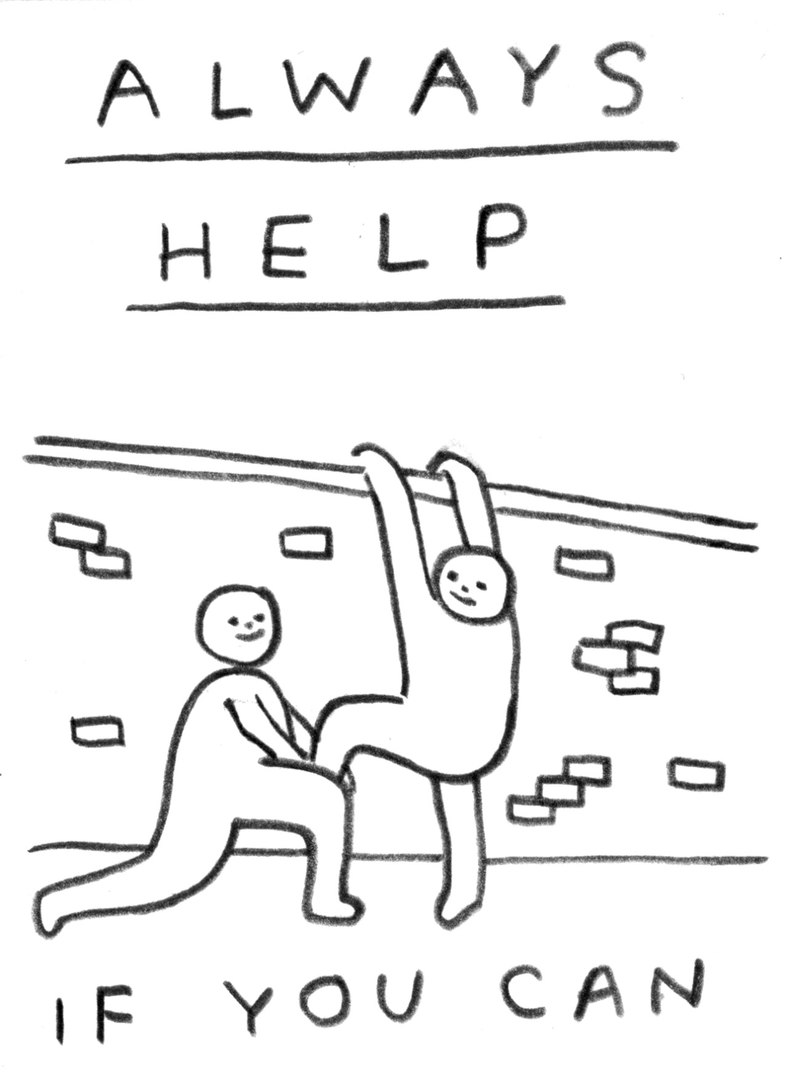
\includegraphics[width=0.23\linewidth]{help.jpg}\\
\ex{}
\end{figure}

\newcounter{j}
\newcommand{\f}[1]{
\addtocounter{j}{1}    
{(       Eq. (\arabic{j}))\\}
#1\\
}
\section{Любимые формулы}

\begin{equation*} 
Var(s)=Var(E(s|r))+E(Var(s|r))  
\qquad{}   \f{}
\end{equation*}
\begin{equation*}
\lim_{n\to 0}(1+x)^{1+x}=\lim_{\alpha\to\infty}(1+\dfrac{1}{\alpha})^{\alpha}=e  
\qquad{}   \f{}
\end{equation*}

 

\end{document}